\chapter{Sequenzdiagramme}

\begin{figure}[H]
  \centering
  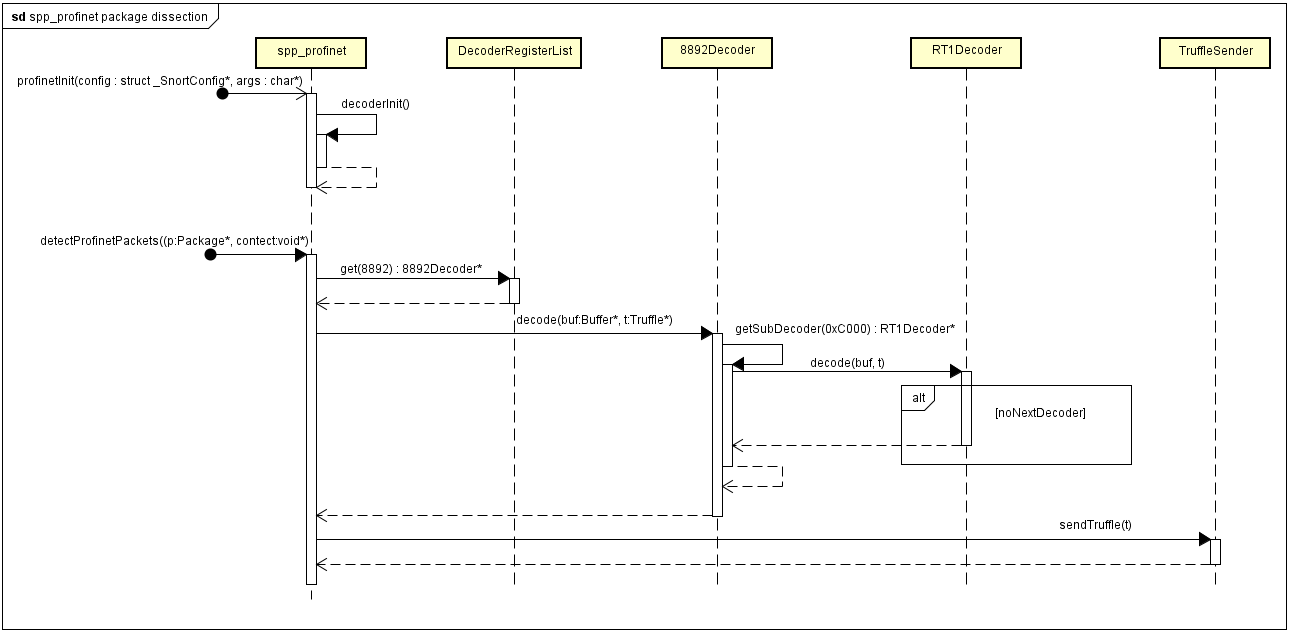
\includegraphics[width=\textwidth]{../diagramimages/spp-profinet-package-dissection.png}
  \caption[Sequenzdiagramm \sppname package dissection]{Sequenzdiagramm \sppname package dissection}
\end{figure}

In dieser Sequenz werden zwei zentrale Aufrufe von \gls{snort} im \gls{praeprozessor} \sppname dargestellt. Zum einen im oberen Teil die Initialisierung des \gls{praeprozessor}s durch einen Init-Aufruf, sowie der \gls{praeprozessor}-interne Aufbau des DecoderRegisters. Dieser Registrierungsvorgang wurde im Diagramm aus Platzgründen eingespaart. Darin wird jeder als C-Datei vorhandene Decoder instanziiert und bei der DecoderRegisterList registriert. Dieser Vorgang legt die Grundlage für den Decoder-Baum-Ablauf, welcher exemplarisch als zweiter unterer Teil des Sequenzdiagramms 